% Emacs settings: -*-mode: latex; TeX-master: "manual.tex"; -*-

\section{Vitess\_ChopperFermi: The Fermi Chopper from Vitess}
\label{s:vit_fc}
\index{Optics!Fermi Chopper}

%\component{Vitess\_ChopperFermi}{Geza Zsigmond}{GeomOption, $N_{\rm chan}$, $f$, $h$, $w_{\rm tot}$, $l$, $r_{\rm curv}$, $d$, $\phi$, $w_{\rm wall}$, GeomFile}{zerotime, $N_{\rm gates}$}{validated}
\mcdoccomp{optics/Vitess_ChopperFermi.parms}


The component {\bf Vitess\_ChopperFermi} simulates a Fermi chopper with absorbing walls.
The shape of the channels can be straight, curved with circular, or curved with ideal
(i.e. close to a parabolic) shape.
This is determined by the parameter 'GeomOption'. In the option 'straight Fermi
chopper', the very fast neutrons are transmitted with only a time modulation and lower
speed neutrons are modulated both in time of flight and wavelength.
If the channels are curved, the highest transmission occurs for a wavelength

\begin{equation}
\lambda_{\rm opt} = \frac{3956 {\rm [m\AA/s]}}{2 \omega r_{\rm curv}}
\end{equation}

with

\begin{equation}
\omega = 2 \pi f
\end{equation}

The optimal shape is calculated in an exact way and is close to parabolic; in this
case, transmission is as high for the optimal wavelength as in the case of a straight
Fermi chopper for the limit $\lambda \rightarrow 0$.
In the more realistic case of circular shapes channels, the transmission is slightly
lower. In general, neutrons are transmitted through a curved Fermi chopper with a time
AND wavelength modulation .

The rotation axis is vertical (y-axis), i.e. the path length through the channels is
given by the length $l$ along the z-axis. The inital orientation is given by the phase
$\phi$ of the chopper - $\phi$ = 0 means transmission orientation.

Geometry for {\bf straight} and {\bf circular} channels:
The geometry of the chopper consists of a rectangular shaped object with a channel
system. In transmission position, there are $N_{\rm gates}$ slits of width $w_{\rm slit}$
each along the x-axis, separated by absorbing walls of thickness $w_{\rm wall}$
(see figure~\ref{f:vit_fc1}). The total width $w_{\rm tot}$ is given by

\begin{equation}
w_{\rm tot} = N_{\rm gates} w_{\rm slit} + (N_{\rm gates}+1) w_{\rm wall}
\end{equation}

The rectangular channel system is surrounded by a so-called shadowing cylinder; it is a
part of a cylinder with vertical symmetry axis and diameter

\begin{equation}
d \geq \sqrt{l^2 + w_{\rm tot}^2}
\end{equation}

It serves to prevent transmission of neutrons which do not fly through the channels;
but it also reduces the transmission, because the cylinder removes neutrons
in front of the channel entrance or behind the channel exit (see figure~\ref{f:vit_fc1}).

\begin{figure}[ht]
\begin{center}
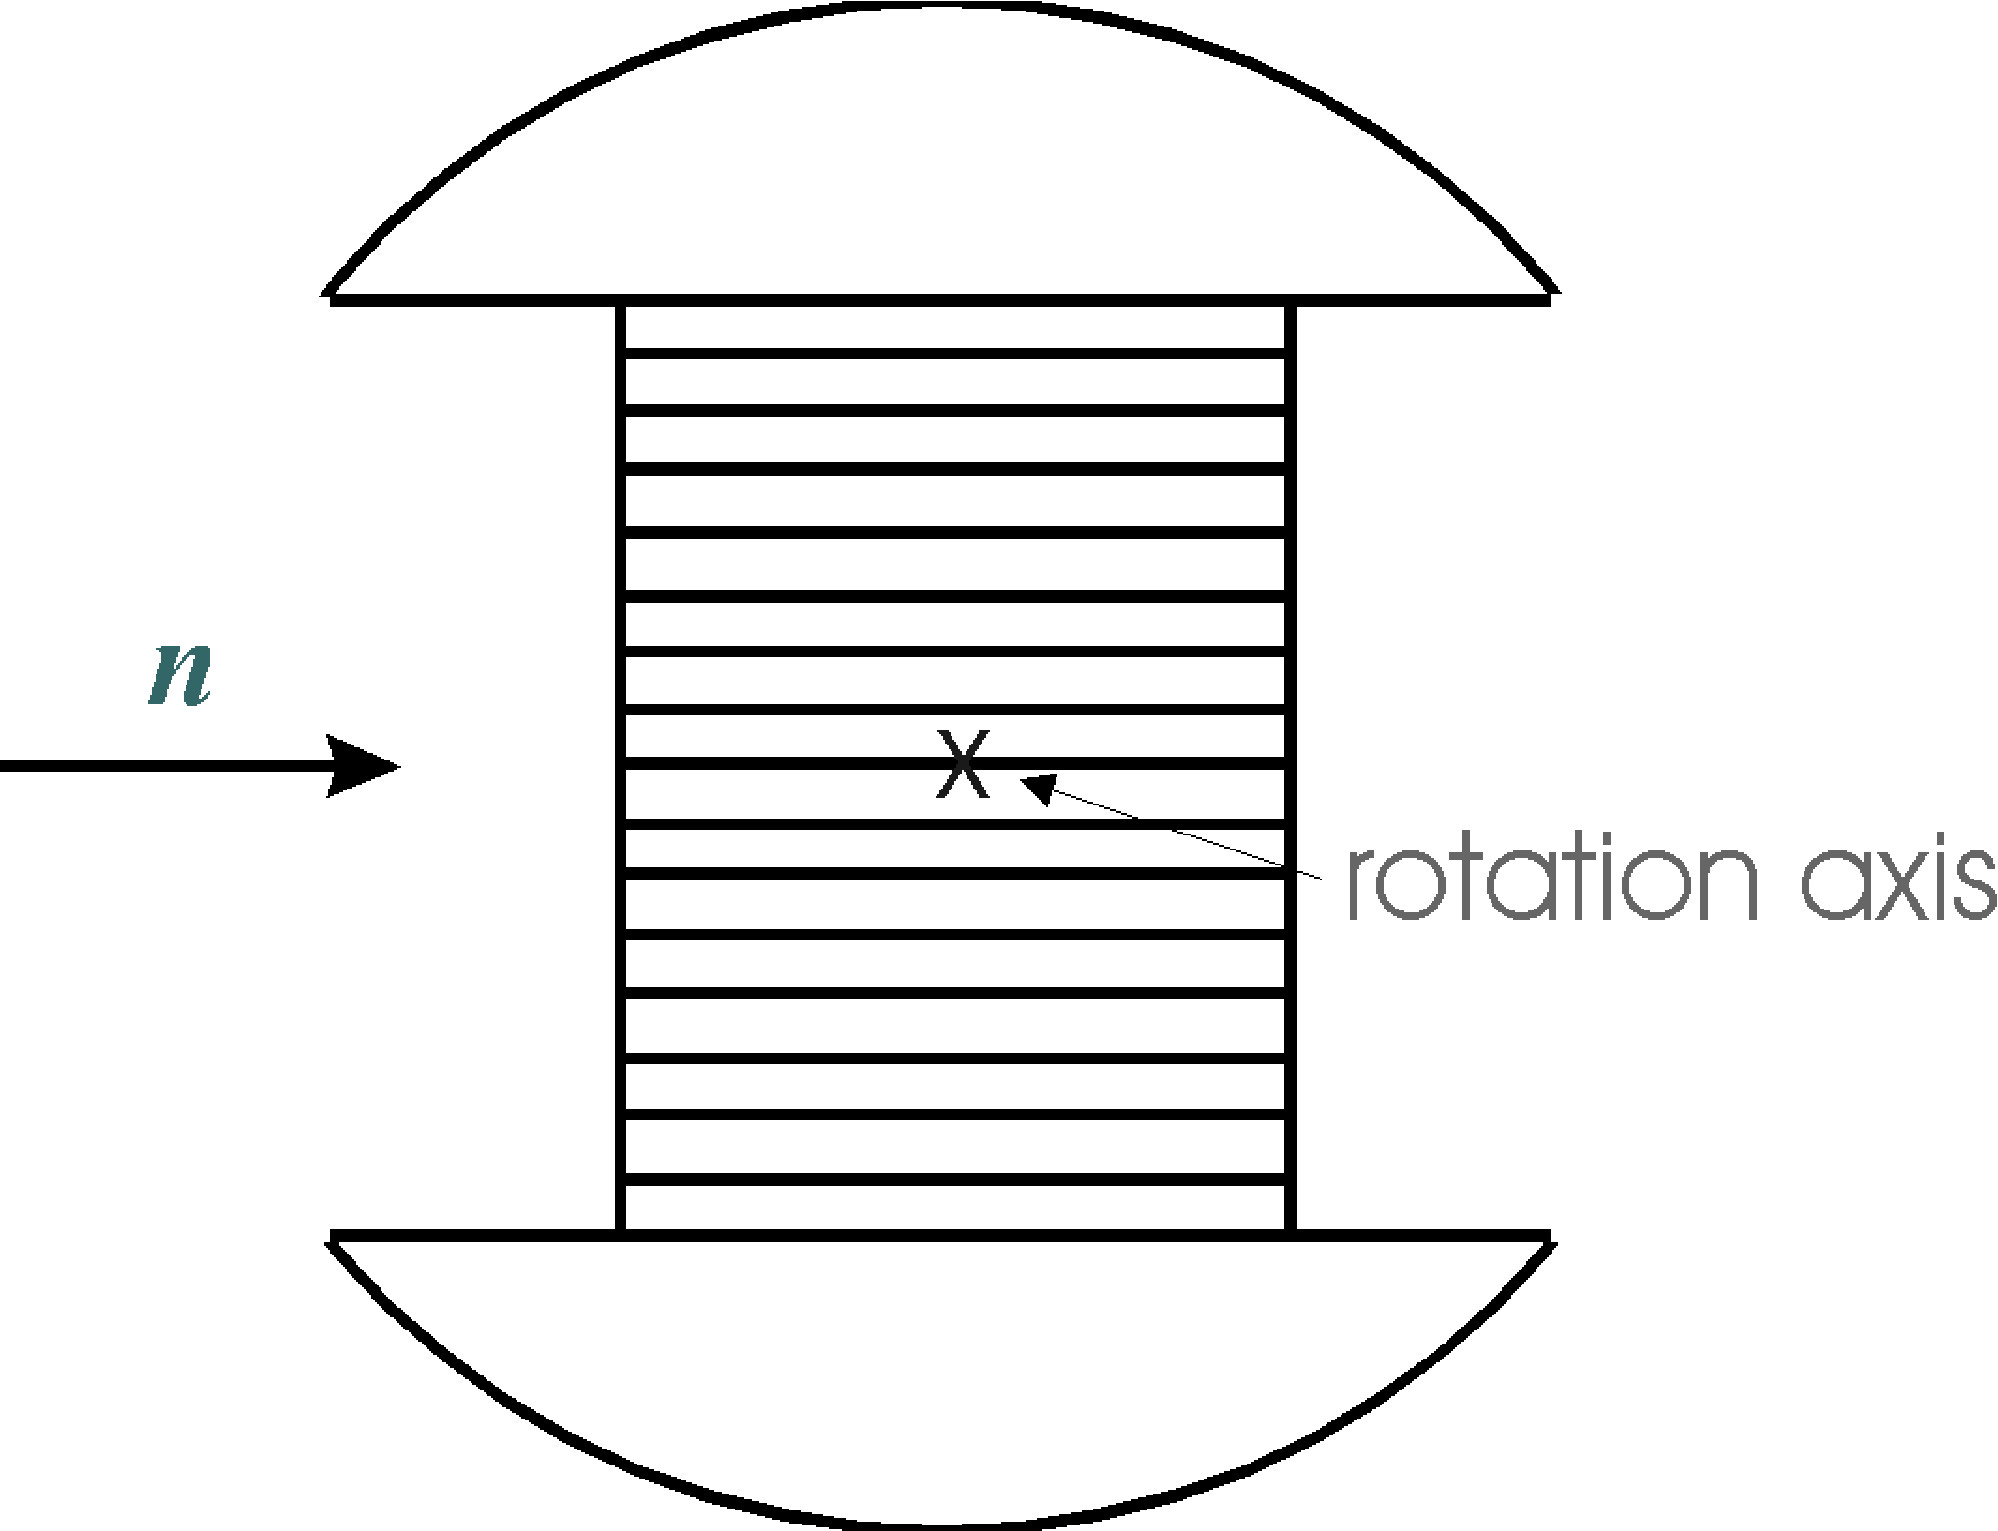
\includegraphics[width=0.45\linewidth]{figures/vitess_fc_str}
\caption{geometry of a staight Fermi chopper\label{f:vit_fc1}}
\end{center}
\end{figure}

Geometry for {\bf parabolic} channels:
In this case, the Fermi chopper is supposed to be a full cylinder, i.e. the central
channels are longer than those on the edges. The other features are the same as for
the other options. (see figure~\ref{f:vit_fc2}).

\begin{figure}[ht]
\begin{center}
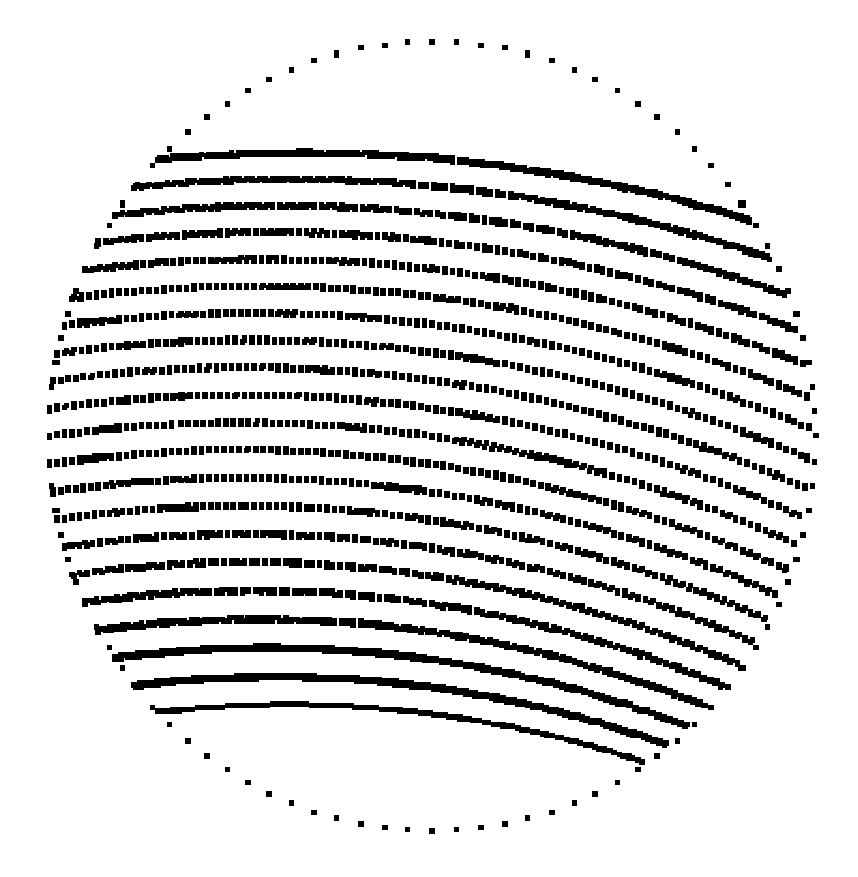
\includegraphics[width=0.4\linewidth]{figures/vitess_fc_parab}
\caption{geometry of a curved Fermi chopper\label{f:vit_fc2}}
\end{center}
\end{figure}

The algorithm works with a rotating chopper framework. Neutrons hitting the channel
walls are absorbed. The channels are approximated by $N_{\rm gates}$ gates. If the trajectory
takes a course through all the gates, the neutron passes the Fermi chopper. There are gates at
the entrance and the exit of the channel. The other gates are situated close to the centre of
the Fermic chopper.
Precision of the simulation increases with the number of gates, but also the computing time needed.
The use of four channels already gives exact transmission shapes for lower wavelengths
($\lambda < 6$ \AA) and good approximation for higher ones. It is recommended to use larger number of
channels only for a check.

The option 'zerotime' may be used to reset the time at the chopper position. The time is
set to a value between -$T_{\rm p}$/2 and +$T_{\rm p}$/2 (with $T_{\rm p}$ being the maximal pulse length),
depending on the phase of the chopper at the moment of passing the chopper centre. The
result is the generation of only 1 pulse instead of several; this is useful for TOF instruments
on continuous sources.

This component is about twice slower than the \verb+FermiChopper+ component.

The component must be placed after a component which sets a non zero flight path to the Fermi Chopper (e.g. not an Arm).
